\documentclass[11pt]{article}
\usepackage{report}

\title{Monte Carlo Methods \\ lab 2}
\author{Jesper Vesterberg (jeve0010@student.umu.se)}

\date{\today}

\begin{document}
\begin{titlepage}
  \maketitle
  \thispagestyle{fancy}
  \lhead{
    Department\\
    Umeå Universitet
  }
  \rhead{\today}
  \begin{abstract}

  \end{abstract}
  \cfoot{
    Numerical Monte Carlo Methods\\
   	Supervisor: Peter Olsson 
  }
\end{titlepage}

\lhead{\theauthor}
\rhead{\thetitle\\\today}
\cfoot{\thepage}



\begin{thebibliography}{9}
\end{thebibliography}

\section{Introduction}
We will look at the scaling phenomena in the Ising model using the wolf-cluster method. This will be done through looking at the magnetization, without an external field, at different temperatures. We will also  look at the binders cumulant. 

\section{Universality}
In figure~\ref{fig:mvsT} we can see how the magnetization is dependent on the temperature, using
the Wolff cluster method. We have different sizes of the system(16, 32, 64, 128 and 256) in order to see how the magnetization changes due to temperature at different system sizes. It can be seen how at larger system we seem to get a clearer jump of magnetization at a certain, critical, temperature.
\begin{figure}[H]
	\centering
	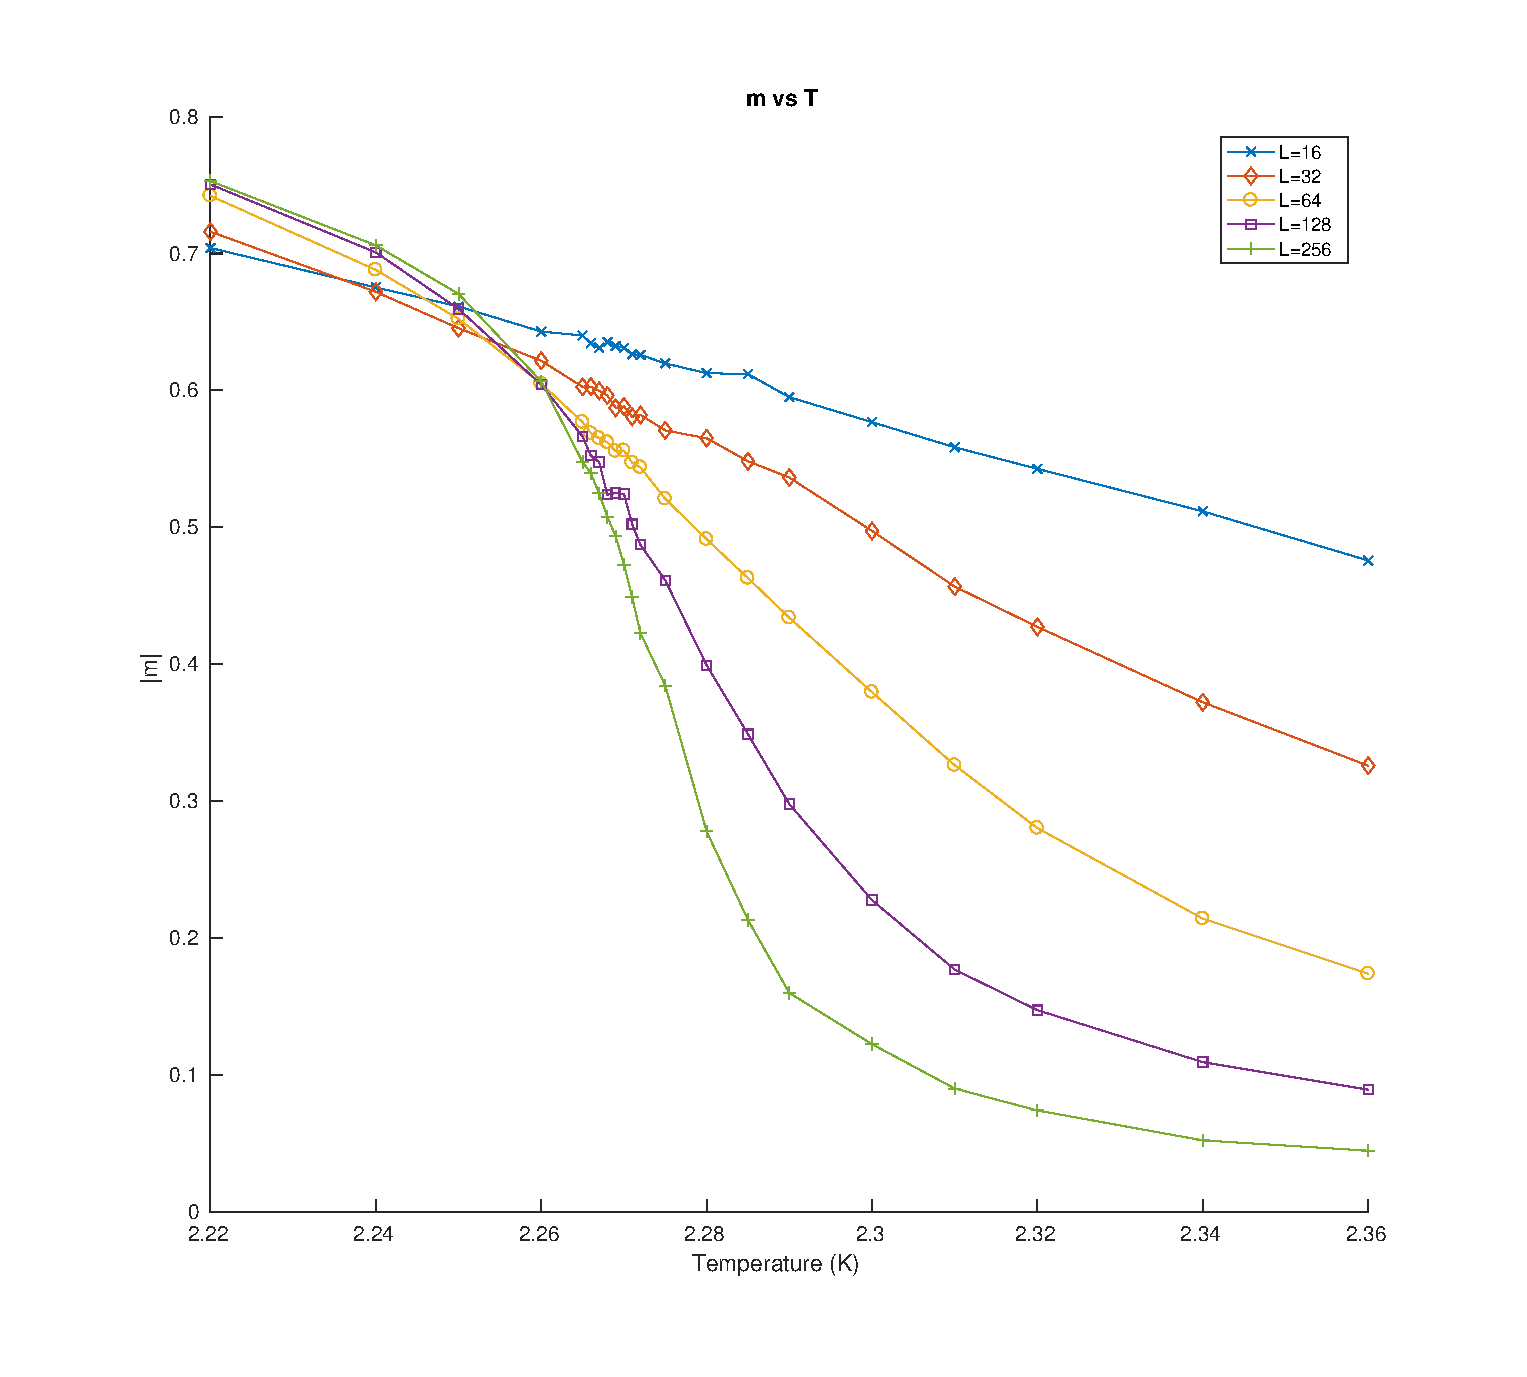
\includegraphics[width=0.9\textwidth]{mvsT}
	\caption{Looking at how the magnetization depends on the temperature for different system sizes using the Wolff cluster
method.}
	\label{fig:mvsT}
\end{figure}

\newpage
In figure~\ref{fig:mlvsT} we can see how we are very close to the correct critical temperature in the
intersection, kind of like how we do with binder’s cumulant. Perhaps this is just an
coincident, perhaps not. It does in anyway clearly show, as in the previous picture, a
clearer drop around the critical temperature for larger systems. We have here used the value of $\beta = 0.125$ and $\nu = 1$.
\begin{figure}[H] 
	\centering
	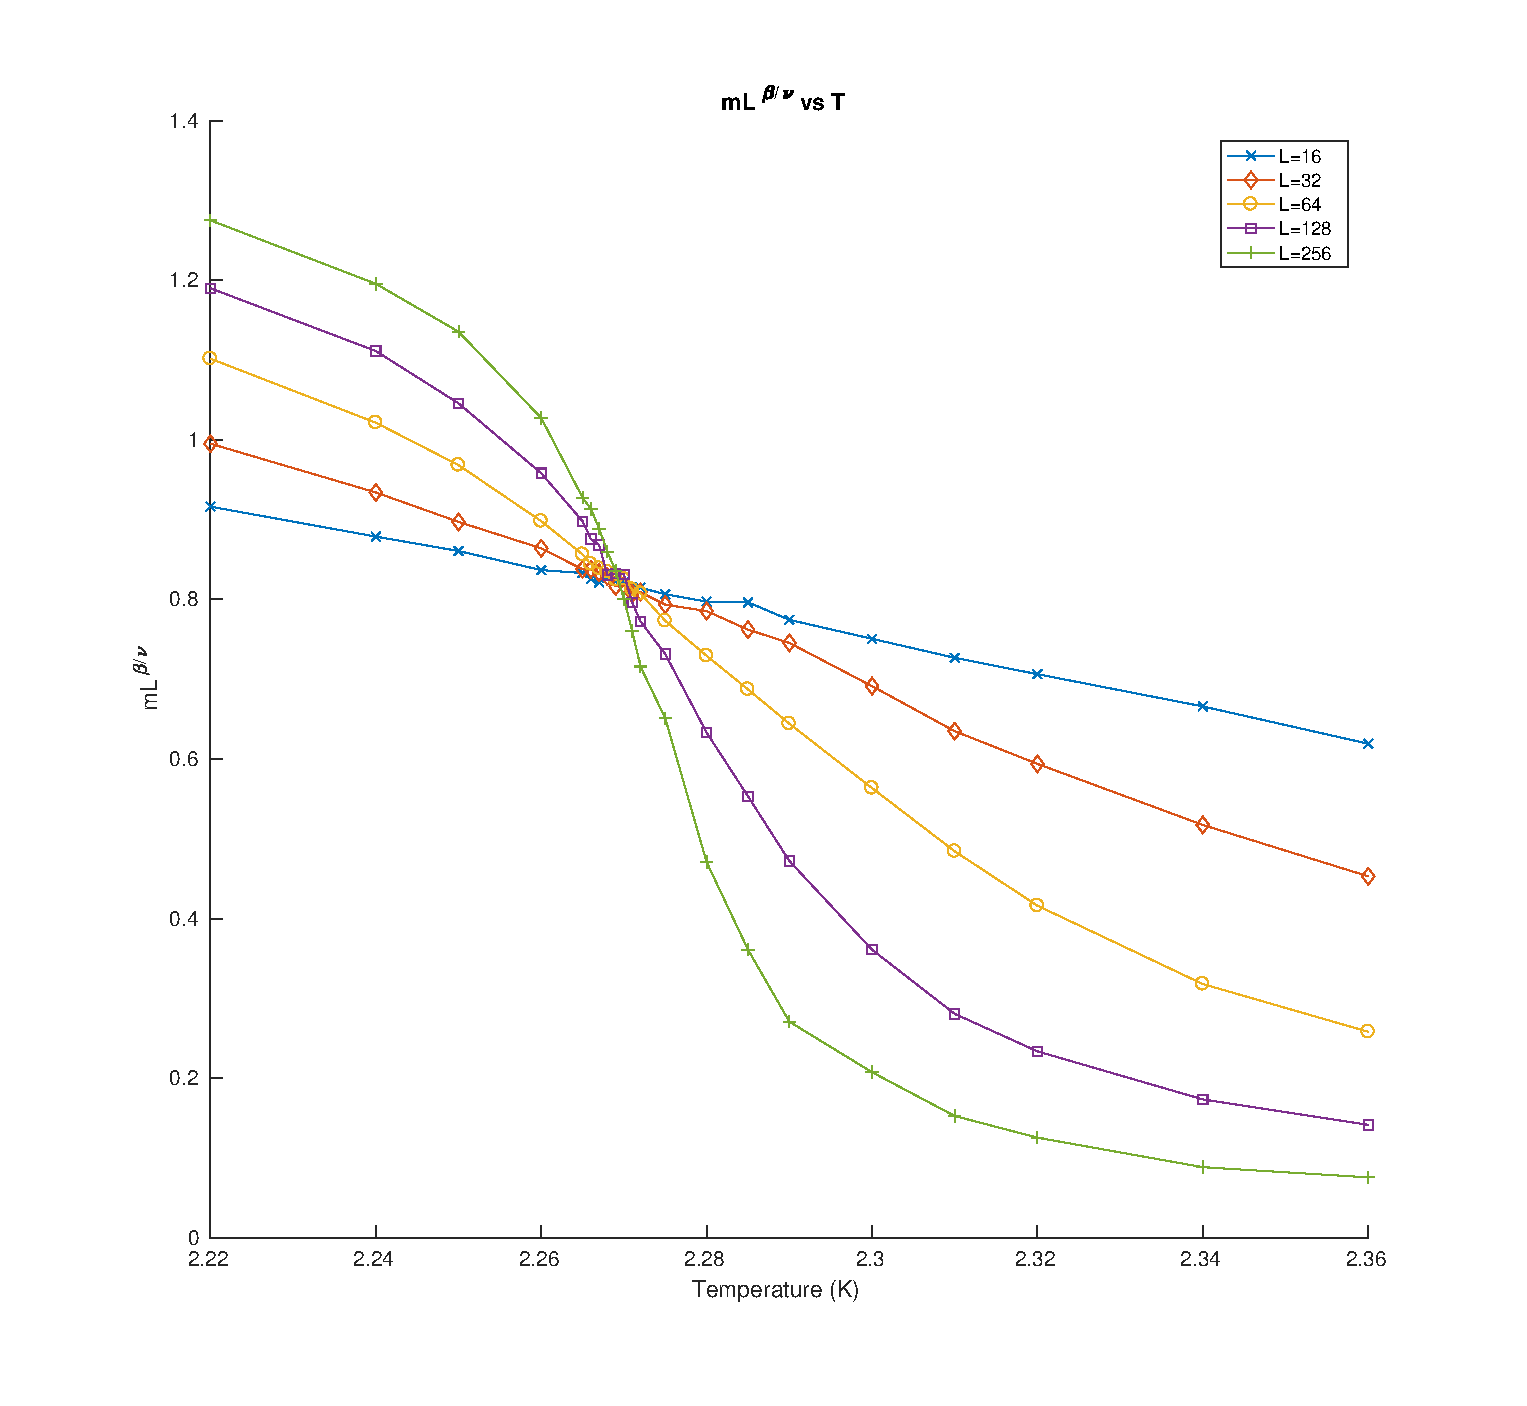
\includegraphics[width=0.9\textwidth]{mlvsT}
	\caption{The scaled magnetization plotted against the temperature}
	\label{fig:mlvsT}
\end{figure}

\newpage
In figure~\ref{fig:mlvstl} we see how the scaling can be used to show you can find the behaviour at
an arbitrary size, when the system has only been simulated for one size. We have used $\beta = 0.125$ and $\nu = 1$ here.
\begin{figure}[H]
	\centering
	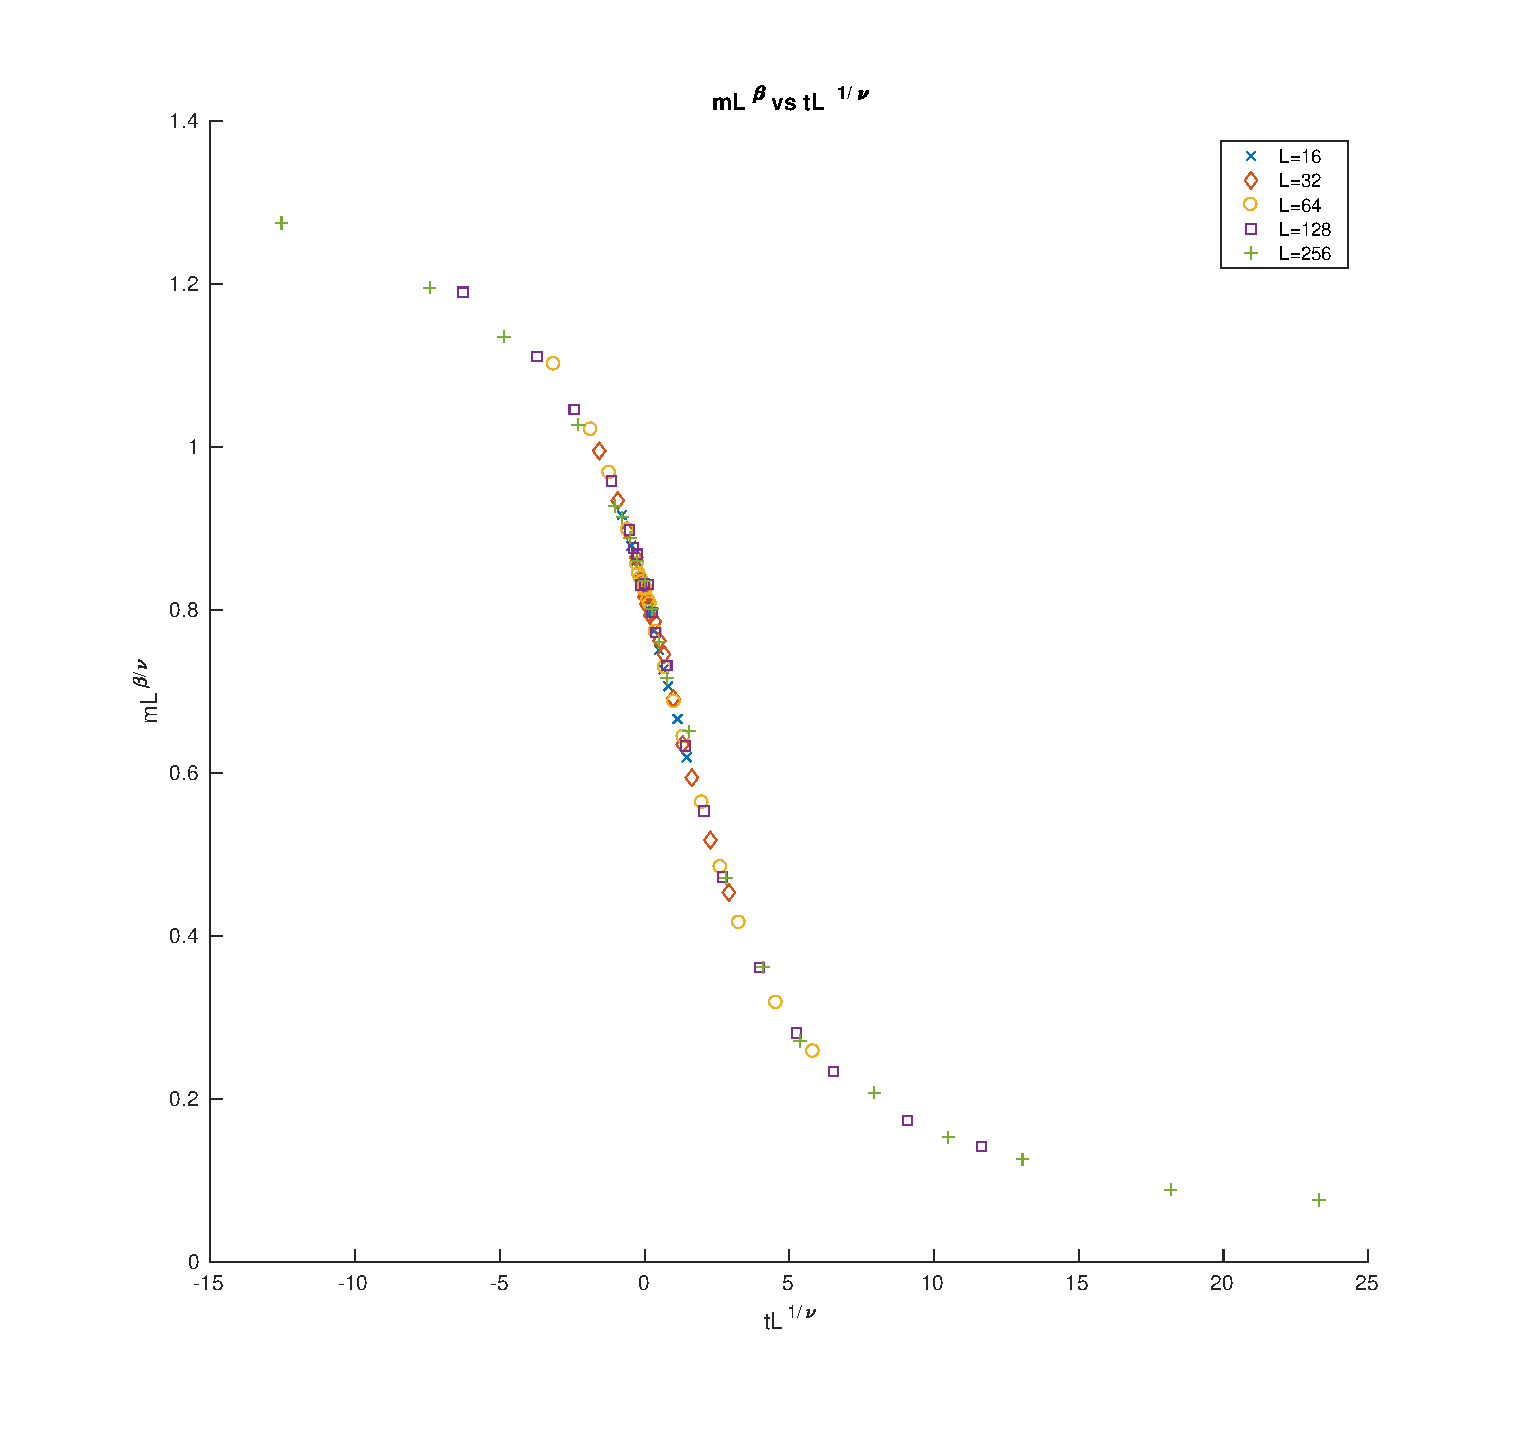
\includegraphics[width=0.9\textwidth]{mlvstl}
	\caption{Using the correct values for the universal constants $\upsilon$ and $\beta$ we get the
characteristic of the different system to collapse ontop of eachother.}
	\label{fig:mlvstl}
\end{figure}

\newpage
In figure~\ref{fig:error} we can see how correct this assumption of the system behaving the same
for all system sizes with the correct scaling. We've zoomed in around the critical temperature and added the error bars in the plot. We still have used $\beta = 0.125$ and $\nu = 1$.
\begin{figure}[H]
	\centering
	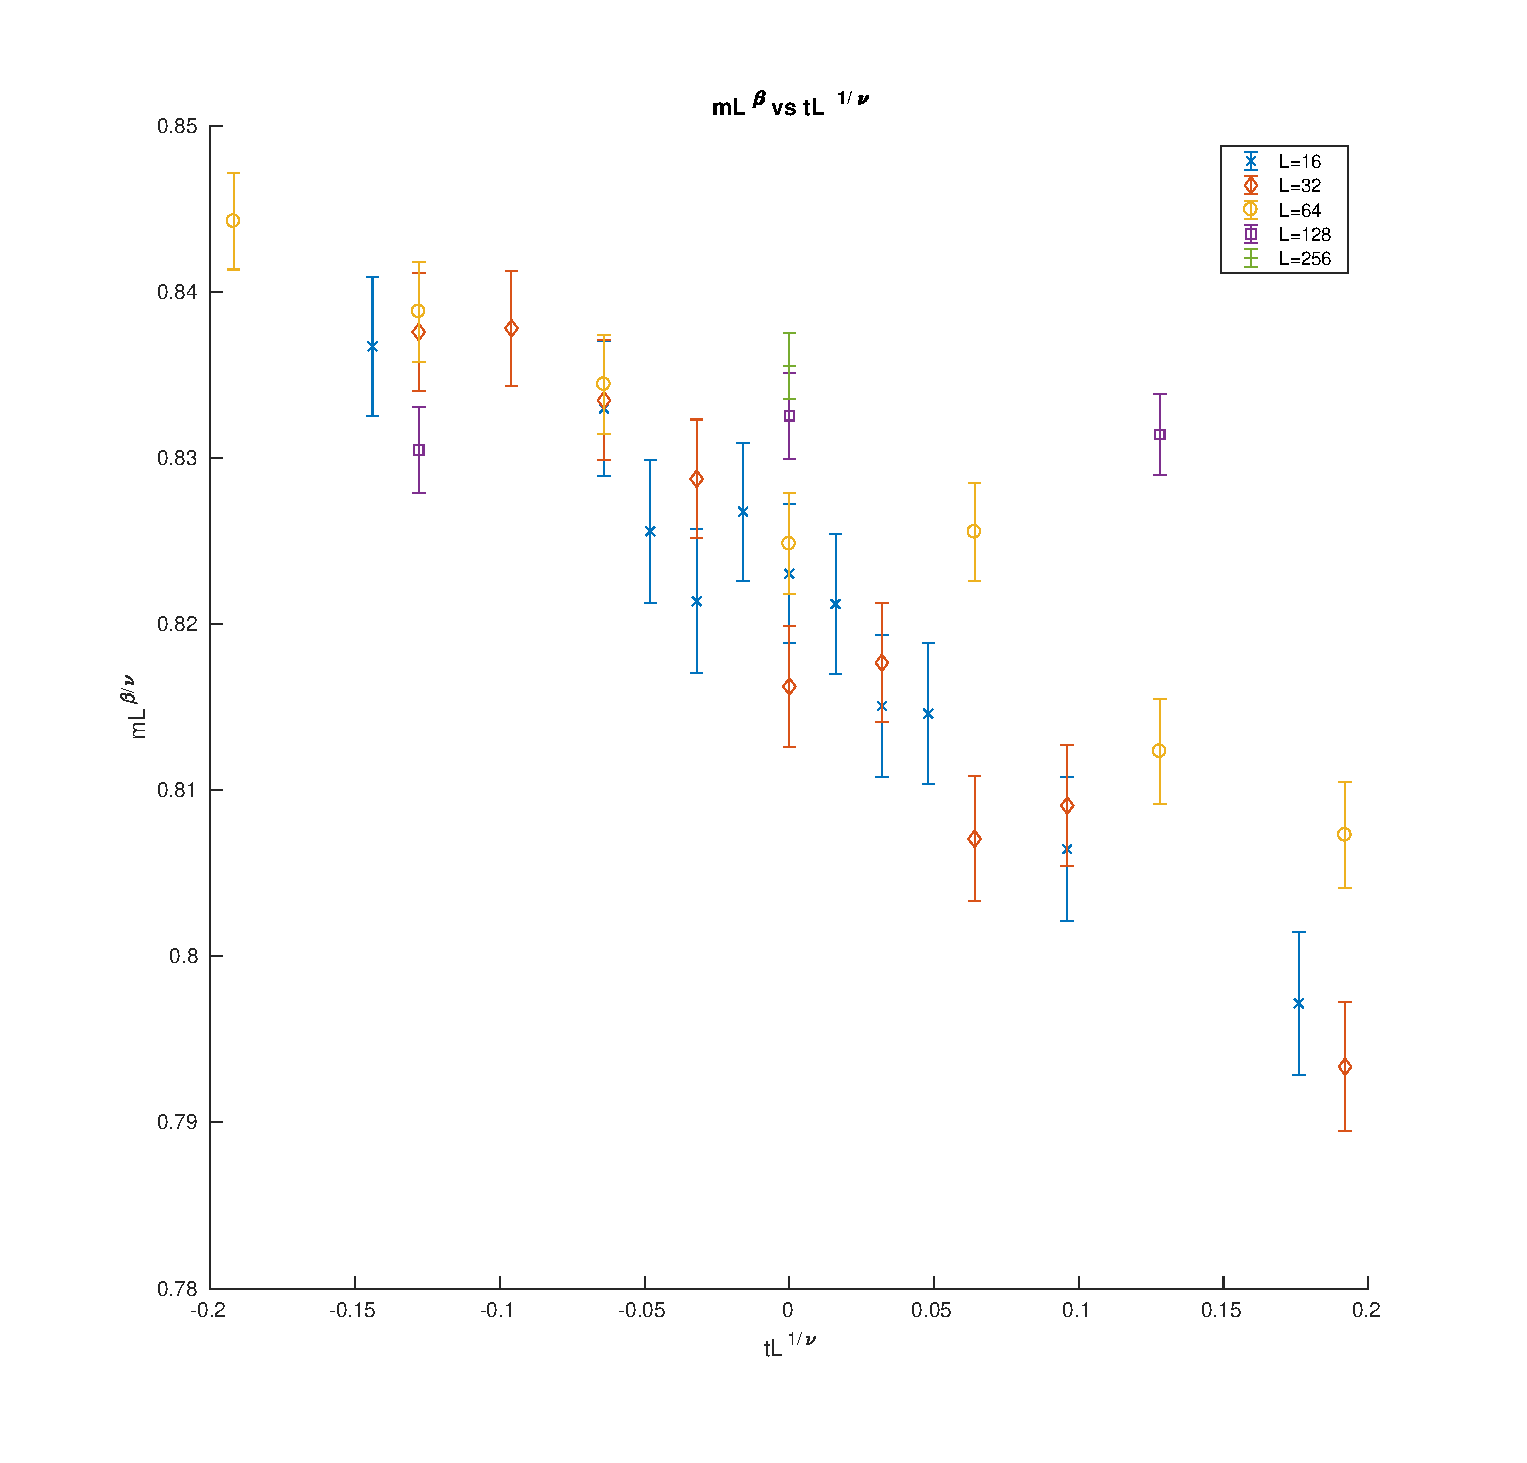
\includegraphics[width=0.9\textwidth]{error}
	\caption{Looking more closely at the collapsed plot in figure~\ref{fig:mlvstl}}
	\label{fig:error}
\end{figure}


\section{Binder's Cumulant}
We now move on to look at binders cumulant
\begin{equation}
	Q_L = \frac{<m^2>^2}{<m>^4}
\end{equation}
where $m$ is the magnetization per spin. We we look around the range $-10 < (t-t_c)L^{1/\nu} <10$.

\newpage
In figure~\ref{fig:cumulant} we can see how Binder's cumulant depends on temperature. From this graph we can get an estimated critical temperature $t_c$ to be around $2.269$.
\begin{figure}[H]
	\centering
	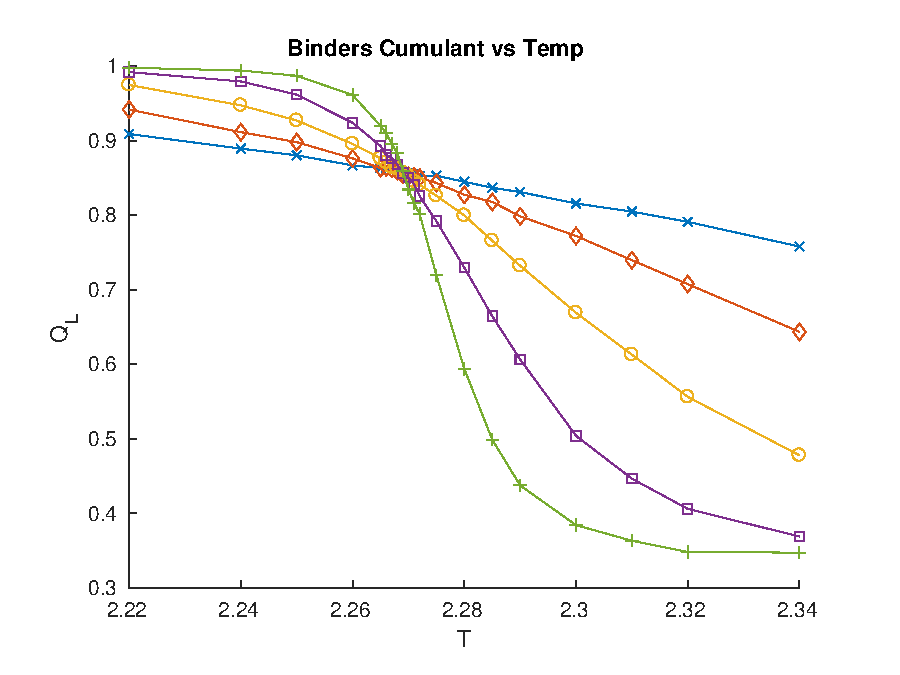
\includegraphics[width=0.9\textwidth]{cumulant}
	\caption{Looking at binder’s cumulant versus temperature to find the critical tempera-
ture.}
	\label{fig:cumulant}
\end{figure}

\newpage
Using the critical value we obtained in figure 5 we can collapse the cumulant function
by plotting in against $(T-T_c)L^{1 / \nu}$, as shown in figure~\ref{fig:scaledtemp}. We're still using $\nu = 1$.
\begin{figure}[H]
	\centering
	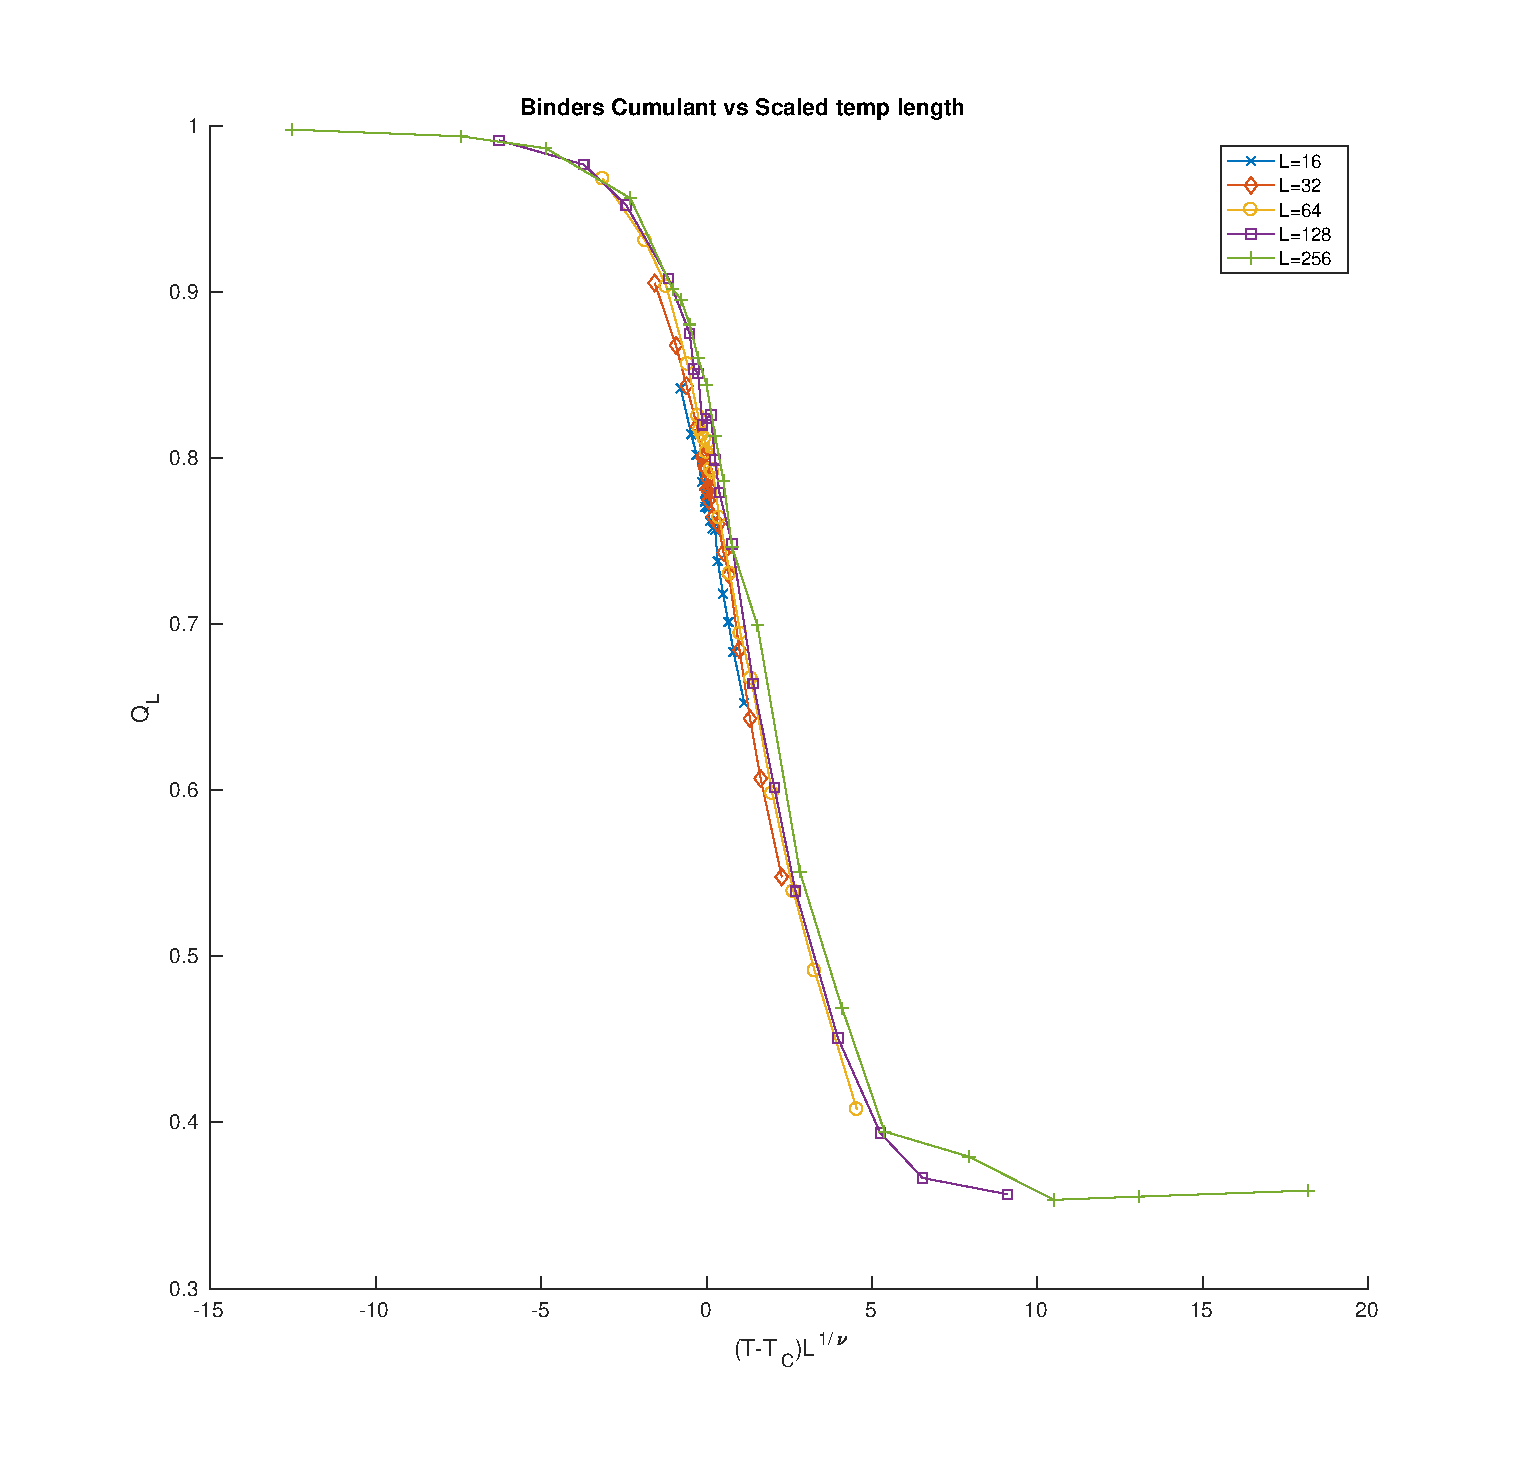
\includegraphics[width=0.9\textwidth]{scaledtemp}
	\caption{Binders cumulant as it depends on the scaled temperature}
	\label{fig:scaledtemp}
\end{figure}
\clearpage
\appendix
\section{Appendix}

\end{document}

